%=-=-=-=-=-=-=-=-=-=-=-=-=-=-=-=-=-=-=-=-=-=-=-=-=-=-=-=-=-=-=-=-=-=- CHAPTER 03
\chapter{Figures \& Images}

%=-=-=-=-=-=-=-=-=-=-=-=-=-=-=-=-=-=-=-=-=-=-=-=-=-=-=-=-=-=-=-=-=-=-=-= SECTION
\section{Storing Images}
It would probably be best if you stored all of your images in a dedicated 
folder.  This will keep your main directory lean in terms of files.
I like to keep my images in a folder called \verb!~/assets!; however, you 
might want to name this to something more creative or appropriate.

To include an image use the \verb!\includegraphics[]{}! command, which accepts 
the file path as its argument and can take multiple options.  It is possible
to include an image anywhere in your document; however, we are
going to place each image in a figure environment that will allow you to both
label and add a caption to your figure that includes your image.

\begin{figure}[h]
    \begin{center}
    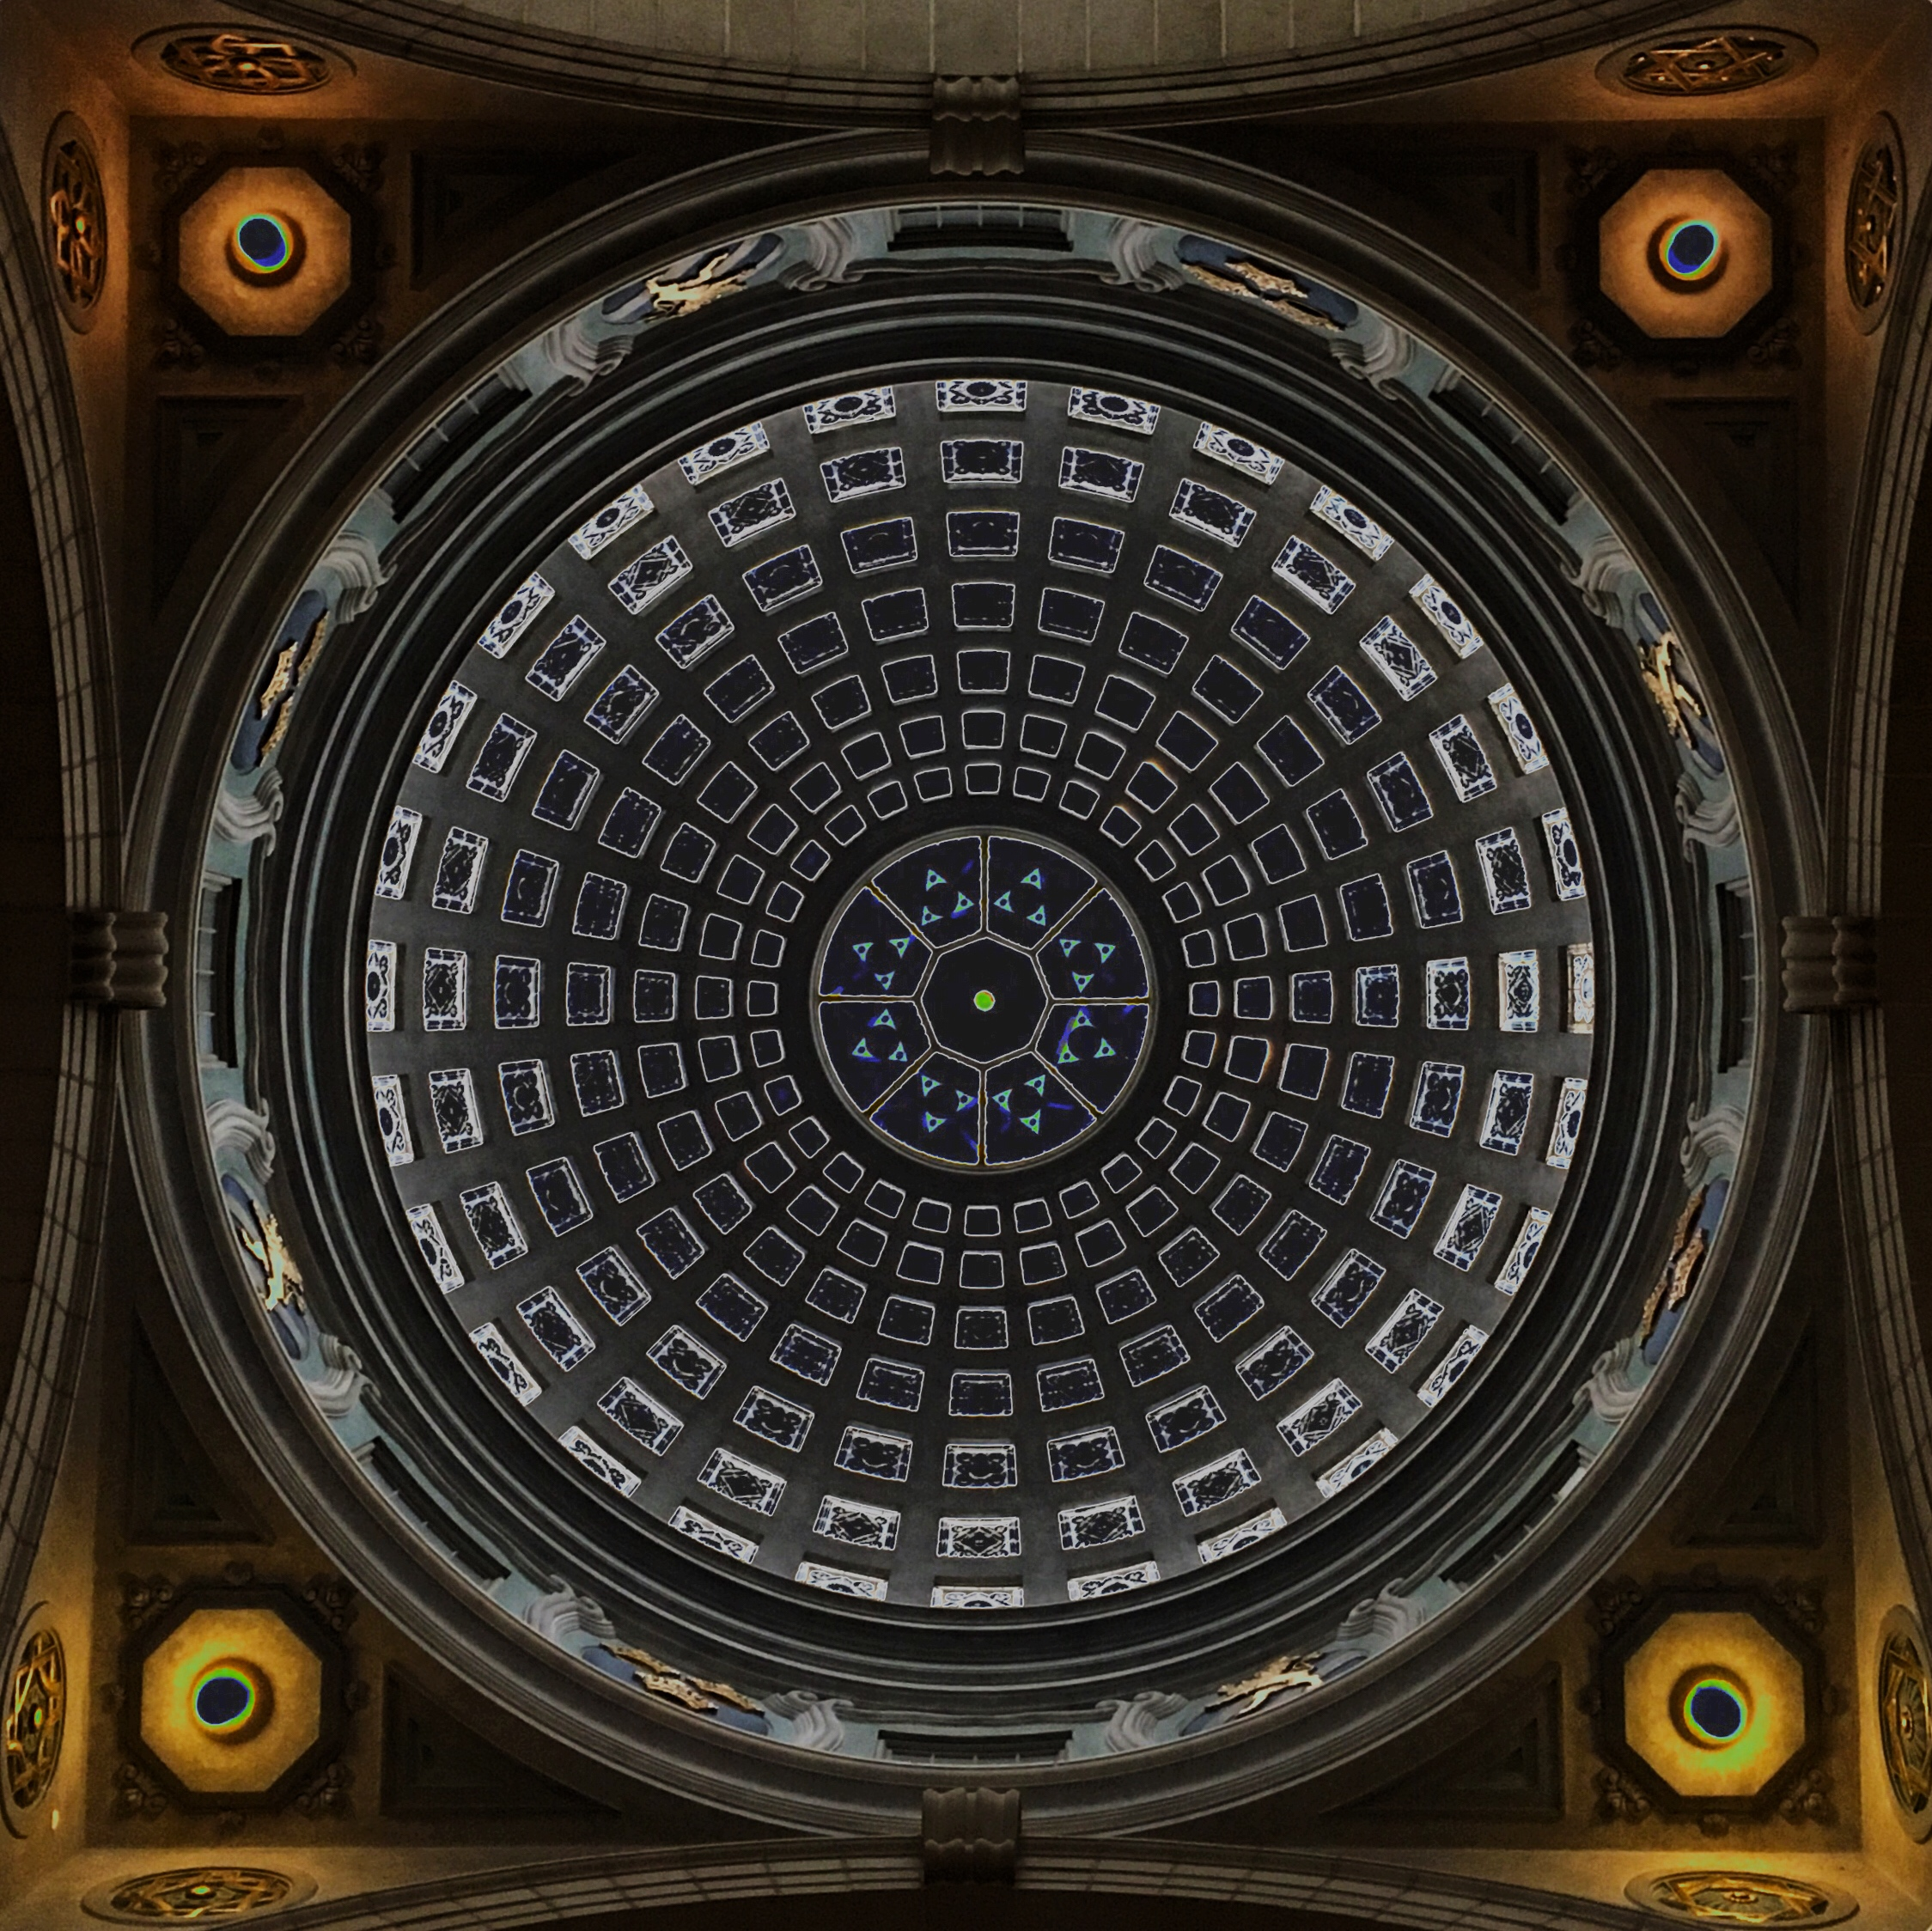
\includegraphics[width = 0.5\textwidth]{image.jpg}
    \end{center}
    \caption{Here is my excellent image.}
    \label{fig:img001}
\end{figure}

Notice how easy it is to reference the above as figure \ref{fig:img001}.

It is also possible to include multiple images that are horizontally aligned
using the subfigure package.

\begin{figure}
    \centering
    \begin{subfigure}[b]{0.3\textwidth}
        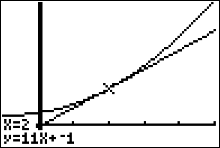
\includegraphics[width=\textwidth]{20170509-123642}
        \caption{Step 1}
        \label{fig:step1}
    \end{subfigure}
    ~ %add desired spacing between images, e. g. ~, \quad, \qquad, \hfill etc. 
      %(or a blank line to force the subfigure onto a new line)
    \begin{subfigure}[b]{0.3\textwidth}
        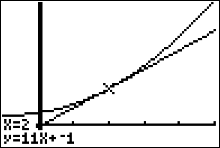
\includegraphics[width=\textwidth]{20170509-123642.png}
        \caption{Step 2}
        \label{fig:step2}
    \end{subfigure}
    ~ %add desired spacing between images, e. g. ~, \quad, \qquad, \hfill etc. 
    %(or a blank line to force the subfigure onto a new line)
    \begin{subfigure}[b]{0.3\textwidth}
        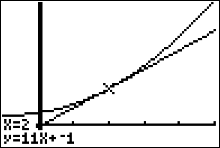
\includegraphics[width=\textwidth]{20170509-123642.png}
        \caption{Step 3}
        \label{fig:step3}
    \end{subfigure}
    \caption{The Steps Shown}\label{fig:threesteps}
\end{figure}